\documentclass{beamer}
\usepackage{amsmath}
\usepackage[english]{babel} %set language; note: after changing this, you need to delete all auxiliary files to recompile
\usepackage[utf8]{inputenc} %define file encoding; latin1 is the other often used option
\usepackage{csquotes} % provides context sensitive quotation facilities
\usepackage{graphicx} %allows for inserting figures
\usepackage{booktabs} % for table formatting without vertical lines
\usepackage{textcomp} % allow for example using the Euro sign with \texteuro
\usepackage{stackengine}
\usepackage{wasysym}
\usepackage{tikzsymbols}
\usepackage{textcomp}
% ELIMINAR COMANDOS DE NAVEGACION%%%%%%%%%%%
\setbeamertemplate{navigation symbols}

%\newcommand{\bubblethis}[2]{
 %       \tikz[remember picture,baseline]{\node[anchor=base,inner sep=0,outer sep=0]%
 %       (#1) {\underline{#1}};\node[overlay,cloud callout,callout relative pointer={(0.2cm,-0.7cm)},%
 %       aspect=2.5,fill=yellow!90] at ($(#1.north)+(-0.5cm,1.6cm)$) {#2};}%
 %   }%
%\tikzset{face/.style={shape=circle,minimum size=4ex,shading=radial,outer sep=0pt,
 %       inner color=white!50!yellow,outer color= yellow!70!orange}}

%% Some commands to make the code easier
\newcommand{\emoticon}[1][]{%
  \node[face,#1] (emoticon) {};
  %% The eyes are fixed.
  \draw[fill=white] (-1ex,0ex) ..controls (-0.5ex,0.2ex)and(0.5ex,0.2ex)..
        (1ex,0.0ex) ..controls ( 1.5ex,1.5ex)and( 0.2ex,1.7ex)..
        (0ex,0.4ex) ..controls (-0.2ex,1.7ex)and(-1.5ex,1.5ex)..
        (-1ex,0ex)--cycle;}
\newcommand{\pupils}{
  %% standard pupils
  \fill[shift={(0.5ex,0.5ex)},rotate=80] 
       (0,0) ellipse (0.3ex and 0.15ex);
  \fill[shift={(-0.5ex,0.5ex)},rotate=100] 
       (0,0) ellipse (0.3ex and 0.15ex);}

\newcommand{\emoticonname}[1]{
  \node[below=1ex of emoticon,font=\footnotesize,
        minimum width=4cm]{#1};}
\usepackage{scalerel}
\usetikzlibrary{positioning}
\usepackage{xcolor,amssymb}
\newcommand\dangersignb[1][2ex]{%
  \scaleto{\stackengine{0.3pt}{\scalebox{1.1}[.9]{%
  \color{red}$\blacktriangle$}}{\tiny\bfseries !}{O}{c}{F}{F}{L}}{#1}%
}
\newcommand\dangersignw[1][2ex]{%
  \scaleto{\stackengine{0.3pt}{\scalebox{1.1}[.9]{%
  \color{red}$\blacktriangle$}}{\color{white}\tiny\bfseries !}{O}{c}{F}{F}{L}}{#1}%
}
\usepackage{fontawesome} % Social Icons
\usepackage{epstopdf} % allow embedding eps-figures
\usepackage{tikz} % allows drawing figures
\usepackage{amsmath,amssymb,amsthm} %advanced math facilities
\usepackage{lmodern} %uses font that support italic and bold at the same time
\usepackage{hyperref}
\usepackage{tikz}
\hypersetup{
    colorlinks=true,
    linkcolor=blue,
    filecolor=magenta,      
    urlcolor=blue,
}
\usepackage{tcolorbox}
%add citation management using BibLaTeX
\usepackage[citestyle=authoryear-comp, %define style for citations
    bibstyle=authoryear-comp, %define style for bibliography
    maxbibnames=10, %maximum number of authors displayed in bibliography
    minbibnames=1, %minimum number of authors displayed in bibliography
    maxcitenames=3, %maximum number of authors displayed in citations before using et al.
    minnames=1, %maximum number of authors displayed in citations before using et al.
    datezeros=false, % do not print dates with leading zeros
    date=long, %use long formats for dates
    isbn=false,% show no ISBNs in bibliography (applies only if not a mandatory field)
    url=false,% show no urls in bibliography (applies only if not a mandatory field)
    doi=false, % show no dois in bibliography (applies only if not a mandatory field)
    eprint=false, %show no eprint-field in bibliography (applies only if not a mandatory field)
    backend=biber %use biber as the backend; backend=bibtex is less powerful, but easier to install
    ]{biblatex}
\addbibresource{../mybibfile.bib} %define bib-file located one folder higher


\usefonttheme[onlymath]{serif} %set math font to serif ones

\definecolor{beamerblue}{rgb}{0.2,0.2,0.7} %define beamerblue color for later use

%%% defines highlight command to set text blue
\newcommand{\highlight}[1]{{\color{blue}{#1}}}


%%%%%%% commands defining backup slides so that frame numbering is correct

\newcommand{\backupbegin}{
   \newcounter{framenumberappendix}
   \setcounter{framenumberappendix}{\value{framenumber}}
}
\newcommand{\backupend}{
   \addtocounter{framenumberappendix}{-\value{framenumber}}
   \addtocounter{framenumber}{\value{framenumberappendix}}
}

%%%% end of defining backup slides

%Specify figure caption, see also http://tex.stackexchange.com/questions/155738/caption-package-not-working-with-beamer
\setbeamertemplate{caption}{\insertcaption} %redefines caption to remove label "Figure".
%\setbeamerfont{caption}{size=\scriptsize,shape=\itshape,series=\bfseries} %sets figure  caption bold and italic and makes it smaller


\usetheme{Boadilla}

%set options of hyperref package
\hypersetup{
    bookmarksnumbered=true, %put section numbers in bookmarks
    naturalnames=true, %use LATEX-computed names for links
    citebordercolor={1 1 1}, %color of border around cites, here: white, i.e. invisible
    linkbordercolor={1 1 1}, %color of border around links, here: white, i.e. invisible
    colorlinks=true, %color links
    anchorcolor=black, %set color of anchors
    linkcolor=beamerblue, %set link color to beamer blue
    citecolor=blue, %set cite color to beamer blue
    pdfpagemode=UseThumbs, %set default mode of PDF display
    breaklinks=true, %break long links
    pdfstartpage=1 %start at first page
    }


% --------------------
% Overall information
% --------------------
\title[Economía I]{Economía I \vspace{4mm}
\\ Magistral 4: La elección del individuo y la curva de demanda individual}
\date{}
\author[Ertola Navajas y Fariña]{Ertola Navajas y Fariña}
\vspace{0.4cm}
\institute[]{Universidad de San Andrés} 


\begin{document}

\begin{frame}
\titlepage
\centering
\includegraphics[scale=0.2]{Slides Principios de Economia/Figures/logoUDESA.jpg} 
\end{frame}

\begin{frame}
\frametitle{¡Retomemos!}
\centering
\includegraphics[scale=0.5]{Slides Principios de Economia/Figures/Tema_02.2_rp.png}
% Copiar imagen que se cambi antes
\end{frame}

\begin{frame}
\frametitle{Tenemos la restricción presupuestaria}
\centering
\includegraphics[scale=0.6]{Slides Principios de Economia/Figures/Tema_02.4_rp2.jpg}
% C6_1.jpg
% O SACAR DE ESTE LAS CANTIDADES EN EJES Y EN Q Y HOMOGENEIZAR O AL REVES, SUMARLO EN LOS OTROS QUE SIGUEN (LOS SIGUIENTES 2)
\end{frame}

\begin{frame}
\frametitle{Agregamos las preferencias}
\centering
\includegraphics[scale=0.6]{Slides Principios de Economia/Figures/Tema_02.18_rp16.jpg}
% C8_1.jpg
\end{frame}

\begin{frame}
\frametitle{Y encontramos el equilibrio}
\centering
\includegraphics[scale=0.6]{Slides Principios de Economia/Figures/Tema_02.19_rp17.jpg}
% C8_2.jpg
\end{frame}

\begin{frame}
\frametitle{Cambios en el precio de la pizza}
\begin{itemize}
    \item Si mantenemos constantes el ingreso del individuo y el precio de la cerveza, ¿cómo afectará un cambio en el precio de la pizza a la cantidad de pizza que adquiera el consumidor? \vspace{2mm}
    \begin{itemize}
         \item La canasta de bienes asequible es la que resulta de igualar la pendiente de la curva de indiferencia con la pendiente de la restricción presupuestaria. 
    \end{itemize}
\end{itemize}
\end{frame}

\begin{frame}
\frametitle{Si aumenta el precio de la pizza:}
\centering
\includegraphics[scale=0.6]{Slides Principios de Economia/Figures/Tema_02.20_rp18.jpg}
% C8_9.jpg SIN B, EL PUNTO B, LA UTILIDAD U2
\end{frame}

\begin{frame}
\frametitle{El nuevo equilibrio es B:}
\centering
\includegraphics[scale=0.6]{Slides Principios de Economia/Figures/Tema_02.22_rp20.jpg}
% C8_9.jpg 
\end{frame}

\begin{frame}
\frametitle{Pensemos un minuto que tenemos aquí...}
\begin{itemize}
    \item Cuando realizamos este ejercicio, estamos obteniendo las cantidades del bien que el individuo está dispuesto a consumir (dado su presupuesto) a cada precio... \vspace{2mm}
    \item Entonces si repetimos el ejercicio varias veces, podríamos ver qué sucede con las cantidades demandadas del consumidor cada vez que el precio aumenta un poquito más.
\end{itemize}
\end{frame}

\begin{frame}
\frametitle{Repitamos el ejercicio de pensar que sucede si cambian los precios... primero el precio es \$50:}
\centering
\includegraphics[scale=0.6]{Slides Principios de Economia/Figures/Tema_02.53_derivacioncurvademanda.png}
\end{frame}

\begin{frame}
\frametitle{Ahora el precio es \$100:}
\centering
\includegraphics[scale=0.6]{Slides Principios de Economia/Figures/Tema_02.54_derivacioncurvademanda1.png}
\end{frame}

\begin{frame}
\frametitle{Y si seguimos aumentando de a \$50...}
\centering
\includegraphics[scale=0.6]{Slides Principios de Economia/Figures/Tema_02.55_derivacioncurvademanda2.png}
\end{frame}

% esta ya no va, hay que borrar
\begin{frame}
\frametitle{Y si seguimos asi...}
\centering
\includegraphics[scale=0.6]{Slides Principios de Economia/Figures/Tema_02.56_derivacioncurvademanda3.png}
\end{frame}

\begin{frame}
\frametitle{¡¡¡Obtenemos la curva de demanda del estudiante!!!}
\centering
\includegraphics[scale=0.6]{Slides Principios de Economia/Figures/Tema_02.57_derivacioncurvademanda4.png}
%C8.18
\end{frame}

\begin{frame}
\frametitle{¿Cómo pasamos de la curva de demanda individual a la curva de demanda del mercado?}
\centering
\includegraphics[scale=0.6]{Slides Principios de Economia/Figures/Demandaagregada.png}
% HACER UNA NUEVA CON LA MISMA ESTRUCTURA QUE LAS DEL TEXTO
\end{frame}

\begin{frame}
\frametitle{Curva de demanda del mercado}
\centering
\includegraphics[scale=0.6]{Slides Principios de Economia/Figures/Tema_02.58_demanda.png}
%C10_4.jpg
\end{frame}

\begin{frame}
\frametitle{¿Qué es la demanda?}
\begin{itemize}
    \item La curva de demanda muestra cuál es la disposición máxima a pagar de los consumidores para cada cantidad del bien, o \vspace{2mm}
    \item ... cuál es la cantidad máxima del bien que está dispuesto a consumir el individuo a cada precio.
\end{itemize}
\end{frame}

% Esta clase sigue en Magistral 9

%%%%%%%%%% SEPARAR CAPITULO 
%%%%%%%%%%%%%%%%%%%%%%%%%%%%%%%%%%%%%%%%%%%%%%%%%%%%%%%%%
%\title[Principios de Economía]{Principios de Economía %\vspace{4mm}
%\\ Capítulo 9: Ocio y Consumo}
%\date{}
%\author[Fariña]{Maximiliano Fariña }
%\vspace{0.4cm}
%\institute[]{Introduzca su nombre aquí} 

%\begin{frame}
%\titlepage
%\centering
%\includegraphics[scale=0.2]{Slides Principios de Economia/Figures/logoUDESA.jpg} 
%\end{frame}
%%%%%%%%%%%%%%%%%%%%%%%%%%%%%%%%%%%%%%%%%%%%%%%%%%%%%%%%%%%%

\begin{frame}
\frametitle{¿Cómo se determina el ingreso?}
\begin{itemize}
    \item Hasta el momento, asumíamos que  conocíamos el ingreso sin preguntarnos como se obtenía. 
    \item Ahora vamos a utilizar las herramientas aprendidas para explicar cómo un individuo determina su ingreso laboral.
    \item A su vez, entender la decisión ocio-trabajo nos será de gran utilidad en la sección de macroeconomía. 
\end{itemize}
\end{frame}


\begin{frame}
\frametitle{Problema consumo - ocio}
\begin{itemize}
    \item Vamos a analizar cómo un individuo decide cuántas horas querrá trabajar por día y, eso definirá su ingreso.
    \item Enfrenta un trade off entre dos bienes: las horas de tiempo libre y el consumo en bienes.
    \item Hay un límite físico: la cantidad de horas por día que puede trabajar o disfrutar.
    \begin{equation}
     24 = H_{Ocio} + H_{Trabajo}.
    \end{equation}
    \item El costo de oportunidad del tiempo libre es el salario. 
    \item El consumo se define por la cantidad de horas de trabajo multiplicado por el salario:
    \begin{equation}
    Consumo = (24-H_{Ocio}) * Salario. 
    \end{equation}
\end{itemize}
\end{frame}


\begin{frame}
\frametitle{Gráficamente..}
\begin{center}
\begin{figure}[H]
\renewcommand{\figurename}{Figure}
\begin{center}
\begin{tikzpicture}[scale=0.6]
\draw[very thick,<->] (0,11) node[left]{Consumo}--(0,0)--(11,0) node[below]{Horas de ocio};
\draw[thin](0,6.5)--(7.5,0);
\draw[thick, dashed,gray] (4.75,2.3)--(4.75,0);
\draw[thick, dashed,gray] (4.75,2.3)--(0 ,2.3);
\node[below] at (4.75,0){\footnotesize 19};
\node[left] at (0,2.3){\footnotesize \$ 50};
\draw[fill] (7.5,0) circle [radius =0.12] node [below] {\footnotesize 24};
\draw[fill] (0,6.5) circle [radius =0.12] node [left] {\footnotesize \$240};
\end{tikzpicture}
\end{center}
\caption{Ocio y consumo}
\label{fig:C6.17}
\end{figure}
\end{center}
\end{frame}

\begin{frame}
\frametitle{La TMS en el modelo ocio - consumo}
\begin{center}
\begin{figure}[H]
\renewcommand{\figurename}{Figure}
\begin{center}
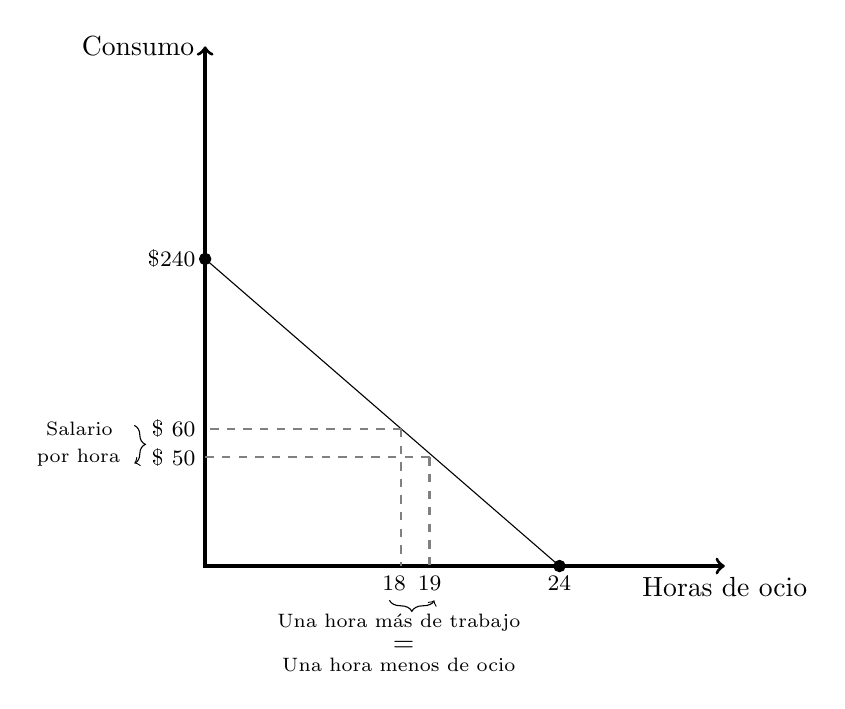
\begin{tikzpicture}[scale=0.6]
\draw[very thick,<->] (0,11) node[left]{Consumo}--(0,0)--(11,0) node[below]{Horas de ocio};
\draw[thin](0,6.5)--(7.5,0);
\draw[thick, dashed,gray] (4.75,2.3)--(4.75,0);
\draw[thick, dashed,gray] (4.75,2.3)--(0 ,2.3);
\draw[thick, dashed,gray] (4.15,2.9)--(4.15,0);
\draw[thick, dashed,gray] (4.15,2.9)--(0 ,2.9);
\node[below] at (4.75,0){\footnotesize 19};
\node[left] at (0,2.3){\footnotesize \$ 50};
\node[below] at (4,0){\footnotesize 18};
\node[left] at (0,2.9){\footnotesize \$ 60};
\draw[fill] (0,6.5) circle [radius =0.12] node [left] {\footnotesize \$240};
\draw [thin,->, decorate,decoration={brace,amplitude=4pt},xshift=0pt,yshift=5pt] (-1.5,2.8) -- (-1.5,2);
\draw [thin,->,decorate,decoration={brace,amplitude=4pt, mirror},xshift=0pt,yshift=5pt](3.9,-0.9) -- (4.85,-0.9);
\draw[fill] (7.5,0) circle [radius =0.12] node [below] {\footnotesize 24};
  \node[left] at (-1.75,2.9){\scriptsize Salario};   
    \node[left] at (-1.6,2.3){\scriptsize por hora};
      \node[] at (4.1,-1.2){\scriptsize Una hora más de trabajo}; 
    \node[] at (4.2,-1.7){=}; 
    \node[] at (4.1,-2.1){\scriptsize Una hora menos de ocio};
\end{tikzpicture}
\end{center}
\caption{Ocio y consumo II}
\label{fig:C6.18}
\end{figure}
\end{center}
\end{frame}

\begin{frame}
\frametitle{El equilibrio}
\begin{center}
\includegraphics[scale=0.6]{Slides Principios de Economia/Figures/C9.4.png}
\end{center}
\end{frame}


\begin{frame}
\frametitle{¿Por qué G no es un equilibrio?}
\begin{center}
\begin{figure}[H]
\renewcommand{\figurename}{Figure}
\begin{center}
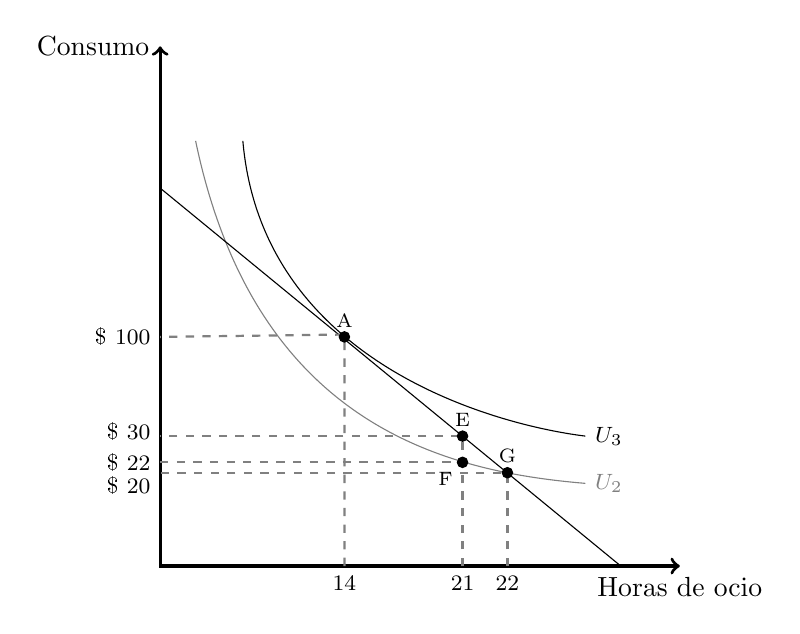
\begin{tikzpicture}[scale=0.6]
\draw[very thick,<->] (0,11) node[left]{Consumo}--(0,0)--(11,0) node[below]{Horas de ocio};
\draw[thin, gray] (0.75,9).. controls (2,3) and (6, 2) .. (9, 1.75) node [right]{\footnotesize $U_2$} ;
\draw[thin] (1.75,9).. controls (2.15,4.35) and (7, 3) .. (9, 2.75) node [right]{\footnotesize $U_3$};
 \draw[thin] (0,8)--(9.75,0) ;
 \draw[thick,gray,dashed] (3.9,0)--(3.9,4.9)--(0,4.85);
%  \draw[thick,gray,dashed] (1.4,0)--(1.4,6.9)--(0,6.9);
% \draw[thick,gray,dashed] (2.2,0)--(2.2,6.2)--(0,6.2); 
\draw[thick,gray,dashed] (6.4,0)--(6.4,2.75)--(0,2.75);
\draw[thick,gray,dashed] (7.35,0)--(7.35,1.975)--(0,1.975);
\draw[thick,gray,dashed] (0,2.195)--(6.4,2.195);
\draw[fill] (3.9,4.85) circle [radius =0.11] node [above] {\scriptsize A};
\draw[fill] (7.35,1.975) circle [radius =0.11] node [above] {\scriptsize G};
\draw[fill] (6.4,2.195) circle [radius =0.11] node [below left] {\scriptsize F};
\draw[fill] (6.4,2.75) circle [radius =0.11] node [above] {\scriptsize E};
% \draw[fill] (1.4,6.9) circle [radius =0.11] node [above] {\scriptsize B};      
% \draw[fill] (2.2,6.2) circle [radius =0.11] node [above] {\scriptsize C};  
% \node[below] at (1.4,0) {\footnotesize 5};
% \node[below] at (2.2,0) {\footnotesize 6};
\node[below] at (3.9,0) {\footnotesize 14};
\node[below] at (6.4,0) {\footnotesize 21};
\node[below] at (7.35,0) {\footnotesize 22};
\node[left] at (0,1.7) {\footnotesize \$ 20};
\node[left] at (0,2.195) {\footnotesize \$ 22};
\node[left] at (0,2.85) {\footnotesize \$ 30};
\node[left] at (0,4.85) {\footnotesize \$ 100};
% \node[left] at (0,6.2) {\footnotesize \$ 900};
% \node[left] at (0,6.9) {\footnotesize \$ 950};
\end{tikzpicture}
\end{center}
\caption{Ocio y consumo II}
\label{fig:C6.23}
\end{figure}
\end{center}
\end{frame}

%AGREGAR SLIDES

% SHOCK DE INGRESO EXTRA FIGURA 9.7

% UN AUMENTO EN EL SALARIO FIGURA 9.8

% EL NUEVO EQUILIBRIO FIGURA 9.9 (EFECTO TOTAL)

% EFECTO INGRESO FIGURA 9.10 (PONER EN GRIS LO QUE NO CORRESPONDE AL EFECTO INGRESO)

% EFECTO SUSTITUCION FIGURA 9.11 (PONER EN GRIS LO QUE NO CORRESPONDE AL EFECTO SUSTITUCION)

% LA CURVA DE OFERTA DE TRABAJO DE LARGO PLAZO
% Texto explicando brevemente que refiera a que se observo en el largo plazo



\end{document}